\documentclass[journal]{IEEEtran}
\usepackage[a5paper, margin=10mm, onecolumn]{geometry}
\usepackage{amsmath,amssymb,amsfonts,amsthm}
\usepackage{gvv-book}
\usepackage{gvv}
\usepackage{hyperref}

\begin{document}

\title{2.10.74}
\author{Puni Aditya - EE25BTECH11046}
\maketitle

\textbf{Question:}\\
If $\vec{X} \cdot \vec{A} = 0$, $\vec{X} \cdot \vec{B} = 0$, and $\vec{X} \cdot \vec{C} = 0$ for some non-zero vector $\vec{X}$, then $\sbrak{\vec{A}\ \vec{B}\ \vec{C}} = 0$.

\textbf{Solution:}\\
Given that for a for a non-zero vector $\vec{X}$:
\begin{align}
    \vec{X} \cdot \vec{A} = 0 \label{eq:1} \\
    \vec{X} \cdot \vec{B} = 0 \label{eq:2} \\
    \vec{X} \cdot \vec{C} = 0 \label{eq:3}
\end{align}

From \eqref{eq:1}, \eqref{eq:2} and \eqref{eq:3},
\begin{align}
    \vec{A}^\top \vec{X} = \vec{B}^\top \vec{X} = \vec{C}^\top \vec{X} = 0
\end{align}
This forms the set of equations
\begin{align}
    \myvec{\vec{A}^\top \\ \vec{B}^\top \\ \vec{C}^\top} \vec{X} &= \myvec{0 \\ 0 \\ 0} \\
    \myvec{\vec{A} & \vec{B} & \vec{C}}^\top\vec{X} &= \vec{0}
\end{align}
For a homogeneous set of equations to have non-trivial solution $\vec{X}$, the coefficient matrix is singular.
\begin{align*}
    \implies \myvec{\vec{A} & \vec{B} & \vec{C}}^\top\text{ is singular.}
\end{align*}
\begin{align*}
    \implies \myvec{\vec{A} & \vec{B} & \vec{C}}\text{ is singular since }\myvec{\vec{A} & \vec{B} & \vec{C}}\text{ is square.}
\end{align*}

\begin{align*}
    \therefore \sbrak{\vec{A}\ \vec{B}\ \vec{C}} = 0
\end{align*}

Hence, the given statement is true. \\

Example: Let
\begin{align*}
    \vec{X}=\myvec{1 \\ 1 \\ 1}, \vec{A}=\myvec{1 \\ -1 \\ 0}, \vec{B}=\myvec{1 \\ 0 \\ -1}, \vec{C}=\myvec{0 \\ 1 \\ -1}
\end{align*}
\begin{align}
    \vec{A}^\top \vec{X} = \vec{B}^\top \vec{X} = \vec{C}^\top \vec{X} = 0\text{ for this example.}
\end{align}
\begin{align}
    \sbrak{\vec{A}\ \vec{B}\ \vec{C}} = \myvec{1 & -1 & 0}\brak{\myvec{1 \\ 0 \\ -1}\times\myvec{0 \\ 1 \\ -1}}
\end{align}
\begin{align}
    \sbrak{\vec{A}\ \vec{B}\ \vec{C}} &= \myvec{1 & -1 & 0} \myvec{1 \\ 1 \\ 1} \\
    \sbrak{\vec{A}\ \vec{B}\ \vec{C}} &= 0
\end{align}

\begin{figure}[h!]
    \centering
    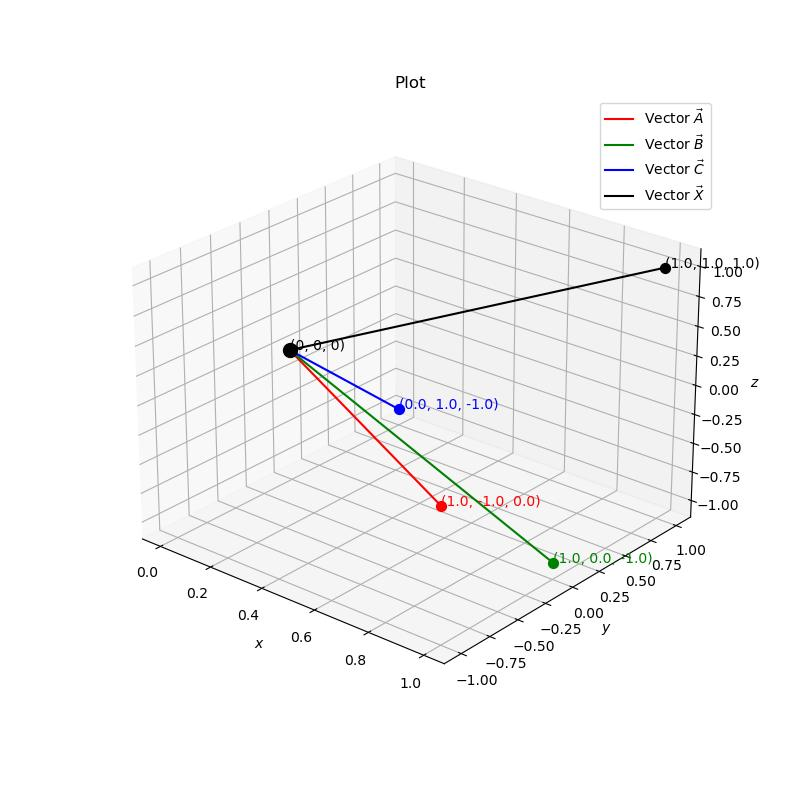
\includegraphics[width=0.7\columnwidth]{figs/plot_c.jpg}
    \caption*{Example}
    \label{fig:fig}
\end{figure}
    
\end{document}
